Machine learning (ML) is the study of algorithms and mathematical models with a feature of progressively improve a performance on a specific task. Machine learning is a subfield of Artificial Intelligence (AI). The main difference between Artificial Intelligence and Machine learning is that machine learning performance results primary depends on the data set and it makes data driven decisions while Artificial Intelligence involves agents at the top. Another subfield of machine learning is Deep Learning that uses a cascade of multiple layers of nonlinear processing units for feature extraction and transformation. Hierarchy representation of Artificial Intelligence, Machine Learning and Deep Learning could be seen in the \ref{fig:ml_hierarchy} figure.

\begin{figure}[H]
\centering
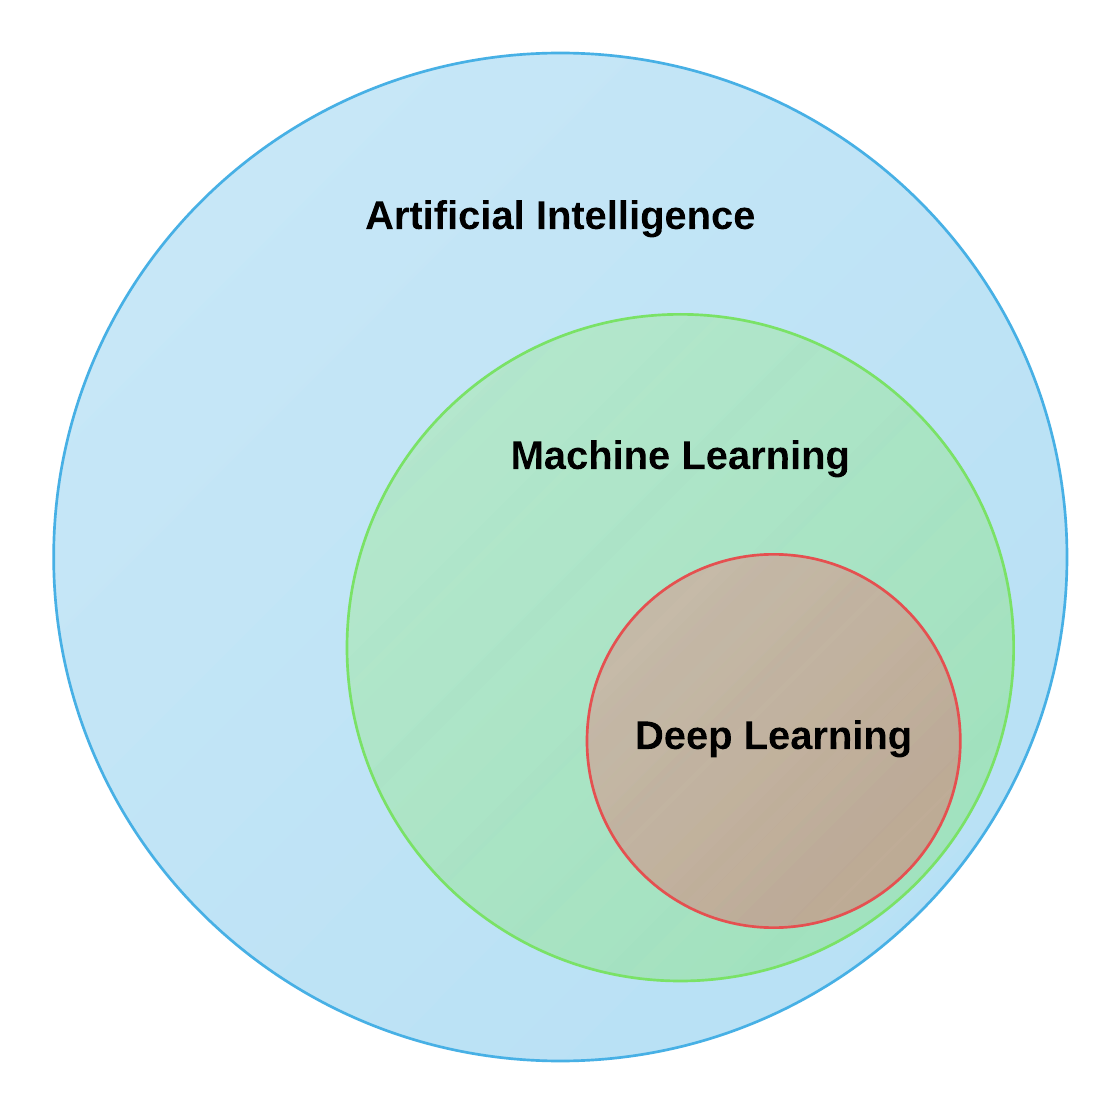
\includegraphics[width=0.5\textwidth]{Pictures/ml_hierarchy.png}
\caption{\label{fig:ml_hierarchy}{}Hierarchy representation of AI, ML and Deep Learning}
\captionsetup{font={footnotesize,bf,it}}
\caption*{Source: https://www.codesofinterest.com/2016/11/difference-artificial-intelligence-machine-learning-deep-learning.html}
\end{figure}


Machine learning models is divided into two types:

\begin{enumerate}
    \item \textbf{Supervised learning} - is the machine learning task of learning a function that maps an input to an output based on example input-output pairs.
    \item \textbf{Unsupervised learning} - is the machine learning tasks that learns from test data that has not been labeled, classified or categorized.
\end{enumerate}




\subsection{Supervised Learning}

Supervised Machine learning models are all about finding appropriate representations for their input data and it requires 3 things:
\begin{enumerate}
    \item \textbf{Input data}. A good data set is the key of creating good Machine Learning model. The input data depends on the problem which the developer want to solve - if the task is speech recognition, then the input data could be sound files converted to the form that computer could proceed, for example: binary. If the task is image tagging, then the data could be a pictures where each pixel is converted to the RGB (red-green-blue) format or HSV (hue-saturation-value) format. The input data depends on the problem and the final goal of the problem. 
    \item \textbf{Output data}. Output data in other words could be called as results of the input data. Supervised machine learning models should know the results of each data input entry point in order to find out a pattern which helps to predict a results. 
    \item \textbf{Validation}. Validation is a way to measure whether the algorithm is doing a good job to determine the distance between the algorithm's current output and its expected output. The validation for supervised machine learning models is split into 2 parts: training data and testing data. Training data is input data and output data which is used for machine learning model training and it from where model learns the patterns of the data which produce certain output. The testing data is used after the machine learning training and from this data the model is evaluated of how successfully it predicted the output results from the input data.
\end{enumerate}


Supervised learning is grouped into two types:

\begin{enumerate}
    \item \textbf{Classification} A classification type is when the output variable is representing a category
    \item \textbf{Regression} A regression type is when the output variable is representing a real value
\end{enumerate}

\subsubsection{Classification}

Classification is the process of predicting the class of given data points. Classes are usually named as a term of \textbf{Labels}. Classification main goal is from given input data points predict an output which would mark a label. Classification predictive modeling: approximating a mapping function (f) from input variables (X) to discrete output variable (y). 


Classification Machine Learning algorithms:

\begin{enumerate}
    \item \textbf{Linear Classifiers} is the statistical classification group of identifying classes of the object's characteristics. A linear classifier methods makes a classification decisions based on the values of a linear combinations of the characteristics. In this paper two linear classifiers would be described: \textit{Logistic Regression} and \textit{Naive Bayes Classifier}
    \begin{enumerate}
        \item \textbf{Logistic Regression}
        \label{sssec:logistic_regression}
        Logistic Regression is a statistical method for analysing a data set in which there are one or more independent variables that determine an measured(outcome) with a dichotomous variable. It predicts the probability of an outcome that have two values. 
        
        The main goal of logistic regression is to find the best fitting model to describe relationship between the dichotomous characteristics of interest and a set of independent variables. 
        
        Logistic regression generates a logistic curve (yellow color) (the Linear and logistic model representation figure \ref{fig:logistic_regression}) which y-axis is limited to values between 0 and 1; [0, 1].
        
        \begin{figure}[H]
            \centering
            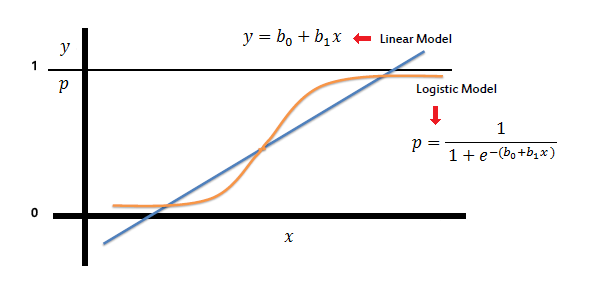
\includegraphics[width=0.8\textwidth]{Pictures/logistic_regression.png}
            \caption{\label{fig:logistic_regression}{} Linear model and Logistic model representation \cite{16}}
        \end{figure}
        
        \textbf{Logistic model} mathematical representation: $p = \frac{1}{1 + e^-(b_{0} + b_{1}x)}$
        
        \textbf{Linear model} mathematical representation: $y = b_{0} + b_{1}x$
        
        \textbf{Logistic regression} could be expressed in the formula:
        
        \begin{equation}
             \frac{p}{1 - p} = \exp{b_{0} + b_{1}x}
        \end{equation}
        \begin{description}
            \item[$p$] Logistic Model 
            \item[$b_{0}$] Logistic regression constant
            \item[$b_{1}$] The slope that defines the steepness of the curve
        \end{description}
        
        \item \textbf{Naive Bayes Classifier}. 
        
        Naive Bayes classifier assumes that the presence of a particular feature in a class is unrelated to the presence of any other feature. Bayes theorem could be expressed in the mathematical equation:
        
        \begin{equation}
                P(A|B) = \frac{P(B|A)P(A)}{P(B)}
        \end{equation}
        \begin{description}
            \item[$A$ and $B$] are events 
            \item[$P(B)$] $\ne 0$
            \item[$P(A | B)$] is a conditional probability: the likelihood of event $A$ occurring given that $B$ is true.
            \item[$P(B | A$] is also a conditional probability: the likelihood of event $B$ occurring given that $A$ is true.
            \item[$P(A)$ and $P(B)$] are the probabilities of observing $A$ and $B$ independently of each other; this is known as the marginal probability
        \end{description}
        
        Naive Bayes \cite{BIB4} is effective in many practical applications including text classification, performance management and medical diagnosis. The effectiveness of Naive Bayes classifier comes from it is presence of feature dependencies: optimality in terms of zero-one loss (classification error) is not necessarily related to the quality of the fit to a probability distribution. 
        
    \end{enumerate}
    \item \textbf{Support Vector Machines(SVM)} 
    
    Support vector machine(SVM) is a discriminative classifier defined by a separating hyperplane. Hyperplane is a line dividing a plane i two parts where in two parts. SVM algorithm main objective is to find a optimal hyperplane in an N-dimensional (N - is the number of features) space that distinctly classifies the data points. 
    
    When using Support Vector Machine it should be considered these parameters:
    
    \begin{itemize}
        \item Input. Set of training pair samples. Call the input sample features $x_{1}, x_{2}...x_{n}$ and the output result y
        \item Output. Set of weights $w$. One for each feature, whose linear combination predicts the value of y
    \end{itemize}
    
    
    
    SVM usage in the real world applications:
    
    \begin{itemize}
        \item Text and Hypertext categorization. SVM method could significantly reduce the need for labeled training instances in both the standard inductive and transductive settings.
        \item Classification of images. SVM achieve higher search accuracy than traditional query refinement schemes
        \item Biological and other sciences. SVM performed good results in classification of proteins schemes or classifying permutation tests.
    \end{itemize}
    
    
    \item \textbf{Decision Trees}
    
    Decision tree are flowchart-like structures that classifies input data points or predict output values given inputs.
    A decision tree is a decision-making device which assigns a probability to each of the possible choices based on the context of the decision: $P(f|h)$, where $f$ is an element of the set of choices and $h$ is the context of the decision. Probability $P(f|h)$ is determined by asking the sequence of questions $q_{1}, q_{2},...,q_{n}$ about the context, where the $ith$ question asked is uniquely determined by the answers to the $i - 1$ previous questions \cite{BIB5}.
    
    
    Decision tree builds classification or regression models in the form of a tree data structure. The data sets is break into smaller subsets. Decisions are represented as nodes and leaf nodes in the tree. 
    
    A decision tree consist of three types of nodes:
    
    \begin{enumerate}
        \item Decision nodes - represented by squares
        \item Chance nodes - represented by circles
        \item End nodes - represented by triangles
    \end{enumerate}
    
    Advantages of Decision trees classification:
    
    \begin{itemize}
        \item Easy to understand and interpret because of the tree structure.
        \item The results could be achieved even with the little data. 
        \item Could determine best, worst and expected values for different scenarios
    \end{itemize}
    
    Disadvantages of Decision trees classification:
    
    \begin{itemize}
        \item It could be unstable. Small changes could imply large changes in the structure of the decision tree
        \item They are often relatively inaccurate comparing with others classification algorithms
        \item Information gain in decision trees is biased in favor of those attributes with more levels
    \end{itemize}
\end{enumerate}

\subsubsection{Regression}

Another type of Machine learning is called Regression. Regression algorithms tries predict a value for an input based on previous information. The main difference of classification type and regression type is that regression main goal is to estimate a value while classification type main goal is to estimate a class of an observation. 

Regression models have the following parameters and variables:

\begin{itemize}
    \item \textbf{The unknown parameters}, denotes as $\beta$, which may represent a scalar or a vector
    \item \textbf{The dependent variable, Y}. This is a main factor that has to be understood and predicted.
    \item \textbf{The independent variables, X}. This is a factor which have an impact on dependent variable
\end{itemize}
A regression model relates Y to a function of X and $\beta$: $Y \approx f(X, \beta)$


Regression Machine Learning algorithms:
\begin{enumerate}
    \item \textbf{Linear Regression}
    
    Linear regression \cite{BIB6} is a technique that analyze the relationships between variables and how they contribute and related to producing a particular outcome. Linear regression establishes a relationship between \textbf{dependent variable (Y)} and \textbf{independent variables (X)} using straight line also known as regression line. 
    
    Linear regression is represented in the formula:
    
    \begin{equation}
     Y = a + b\times X + e
    \end{equation}
    \begin{description}
        \item[Y] Dependent variable 
        \item[X] Independent variables
        \item[a] Intercept
        \item[b] Slope
        \item[e] Error term
    \end{description}
    This equation represents of how Linear Regression method predicts value of target variable on given predictor variables.
    
    Example of the linear regression scatter plot could be seen in the figure \ref{fig:linear_regression}. The black line consists of the predictions, the points are the data and the vertical lines between the points and  the black line represent errors of prediction.
    \begin{figure}[H]
        \centering
        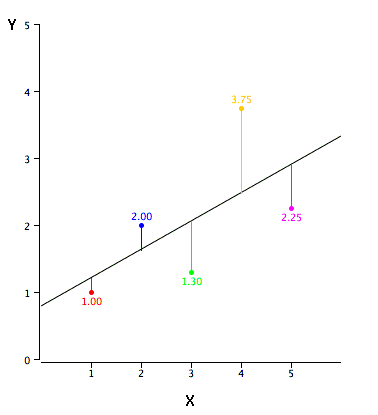
\includegraphics[width=0.55\textwidth]{Pictures/linear_regression.png}
        \caption{\label{fig:linear_regression}{}Scatter plot of the linear regression method \cite{BIB17}}
    \end{figure}
    
    
    Logistic regression \tectbg{properties}:
    
    \begin{itemize}
        \item Linear regression method requires linear relationship between independent variable (Y) and dependent variables X
        \item Linear regression results could be drastically dependent on Outliers. Outliers are the Data points that diverge in a big way from the overall pattern. 
        \item Multicollinearity could increase the variance of the coefficient estimates and make the estimates sensitive to minor changes in the model. Multicollinearity is a statistical process in which predictor variables are correlated.
    \end{itemize}
    
    \textbf{Advantages} of using logistic regression model:
    
    \begin{itemize}
        \item Space complexity of the logistic regression model is low because it needs only to save the weights at the end of training
        \item Good interpretability, simple to understand
        \item Feature importance is generated at the time model building. Dimensionality reduction could be achieved by handling feature selection and by using hyperparameters 
    \end{itemize}
    
    \textbf{Disadvantages} of using logistic regression model:
    
    \begin{itemize}
        \item Multicollinearity should be avoided
        \item Prone to outliers
        \item Linear regression assumes that the data is independent
    \end{itemize}
    
    \item \textbf{Polynomial Regression}
    
    Polynomial Regression method is the relationship between the \textbf{independent variables X } and the \textbf{dependent variable Y} which is modelled as an $nth$ degree polynomial. This method is good for handling non-linearly separable data. This method fits a nonlinear relationship between the value of x and the corresponding conditional mean of Y, denoted as $E(Y|X)$. 
    
    $nth$ degree polynomial regression method could be described in the mathematical formula:
    \begin{equation}
     Y = \beta_{0} + \beta_{1}x + \beta_{2}x^2 + \beta_{3}x^3 + ... + \beta_{n}x^n + e
    \end{equation}
    \begin{description}
        \item[Y] Dependent variable 
        \item[x] Independent variables
        \item[$\beta$] Unknown parameters
        \item[e] Error term
    \end{description}
    
    Polynomial regression properties:
    \begin{itemize}
        \item Otherwise than linear regression, polynomial regression method could model non-linearly seperable data
        \item Full control over the modelling of feature variables
        \item Prone to over fitting if exponents are not selected according to model design.
    \end{itemize}
    
    Polynomial regression have few problems that should be taken to consideration before using this algorithm:
    \begin{enumerate}
        \item When the X values are large, the model could be leaded to the math overflow which could make results inaccurate.
        \item The parameters of the model are intertwined so that lead=s of having covariance and dependency cases between the X values.
    \end{enumerate}
    
    \item \textbf{Ridge Regression}
    
    Ridge regression is a remedial measure taken to alleviate multicollinearity amongst regression predictor variables in a model. By adding a degree of bias to the regression estimates, ridge regression reduces the standart errors rate. 
    
    Ridge regression model formula:
    \begin{equation}
     Y = X\beta + e
    \end{equation}
    \begin{description}
        \item[Y] Dependent variable 
        \item[X] Independent variables
        \item[$\beta$] Regression coefficients to be estimated
        \item[e] Error term
    \end{description}
    
    
    The presence of multicollinearity could be detected in a few ways:
    \begin{itemize}
        \item A regression coefficient is not significant even though variables should be correlated with dependent variable Y
        \item The regression coefficients changes dramatically if X independent variables are added or deleted
        \item X independent variables have high pairwise correlations
    \end{itemize}
    
    Features of ridge regression model:
    \begin{itemize}
        \item The assumption is the same as least squared regression
        \item The value of coefficients does not reach zero
    \end{itemize}
    
    
    \item \textbf{Lasso Regression}
    
    Lasso regression \cite{BIB7} method performs both variable selection and regularization in order to enhance the prediction. Lasso regression and ridge regression are similar methods but lasso regression is using an absolute value bias while ridge regression method is using squared value bias.
    
    The goal of lasso method is to obtain the subset of predictors that minimizes prediction error for a quantitative response variable. This is done by shrinking variables towards zero.
    
    The lasso estimate is defined by formula:
    
    $\beta^{\mathit{lasso}} = argmin \sum_{i=1}^N(y_{i} - \beta{0} - \sum_{j=1}^P x_{ij}\beta_{j})^2$ subject to $\sum_{j=1}^P |\beta_{j}| <= t$ 
    
    Lasso regression translates each coefficient by a constant factor $\lambda$, truncating at zero. This process is called "soft thresholding," and is used in the context of wavelet-based smoothing.
    
    Lasso regression is often an effective technique for shrinkage and feature selection.
    
\end{enumerate}


\subsection{Unsupervised Learning}

Unsupervised machine learning clusters only need to have an input data which would be used for detecting a patterns of the data.  

\subsubsection{Clustering}

Clustering is a task of grouping a set of objects by their data property patterns. Clustering methods are used for identifying similar groups to entities of that group than those of the other groups. Clustering methods are diverse by their types:
\begin{enumerate}
    \item \textbf{Centroid-based}
    
    Clustering model which is related to the notion of similarity is derived by the closeness of a data point to the centroid of the clusters. Using algorithms with this type it is important to know the number of clusters before grouping data.
    
    \item \textbf{Distributed-based}
    
    Clustering model which is based on the notion of how probable is it that all data points in the cluster belong to the same distribution. Distributed-based models tends more suffer from overfitting. 
    
    \item \textbf{Connectivity-based}
    
    Clustering model which is based on the notion that the data points closer in data space exhibit more similarity to each other than the data points lying farther away. This model could be diverse into two approaches:
    \begin{enumerate}
        \item Classifying all data points into separate clusters and then aggregating them as the distance decrease.
        \item All data points are classified as a single cluster and then partitioned as the distance increases.
    \end{enumerate}
    Models are very easy to interpret but lacks scalability for handling big data sets
    
    \item \textbf{Density-based}
    
    Clustering model which is search the data space for areas of varied density of data points in the data space. It isolates various different density regions and assign the data points within these regions in the same cluster.
    
\end{enumerate}


\begin{enumerate} 

    \item \textbf{K-Means Clustering}
    
    K-mean is a centroid model based clustering algorithm which the main goal is to partition the inputs into sets $S1,...,S_{k}$ in a way that minimizes the total sum of squared distances from each point to the mean of its assigned cluster. $k$ representing the number of clusters. 
    
    K-means \cite{BIB8} clustering abstract algorithm:
    
    \begin{enumerate}
        \item Decide on a value for K, the number of clusters
        \item Initialize the K cluster centers 
        \item Decide the class memberships of the N objects by assigning them to the nearest cluster center
        \item Re-estimate the K cluster centers, by assuming the memberships found above are correct
        \item Repeat c and d until none of the N objects changed membership in the last iteration
    \end{enumerate}
    
    \textbf{Advantages} of K-mean clustering :
    \begin{itemize}
        \item K-mean clustering is fast. Computing the distances between points and group centers requires few computations. The linear complexity of the algorithm is \textbf{O(n)}
        \item An instance could move to another cluster when the centroids are recomputed
        \item Converges to local minimum of within-cluster squared error
    \end{itemize}
    
    
    \textbf{Disadvantages} of K-mean clustering:
    \begin{itemize}
        \item The exact number of clustering groups/classes should be known before using k-means clustering algorithm 
        \item K-means starts with a random choice of cluster centers and it could perform different results for each algorithm run
        \item The order of the data has an impact to the final results
        \item Sensitive to outliers
        \item Detects spherical clusters only
    \end{itemize}
    
    
    \item \textbf{Mean-Shift Clustering}
    
    Mean-shift \cite{BIB9} clustering algorithm is a non parametric clustering technique which does not require prior knowledge of the number of clusters and does not constrain the shape of the clusters. 
    
    
    \begin{equation}
        K(x) = 
        \left \{
          \begin{tabular}{ccc}
          1 if ||x|| <= \lambda \\
          0 if ||x|| > \lambda 
          \end{tabular}
        \right \}
    \end{equation}
    \begin{description}
         Let data be a finite set $S$ embedded in the n-dimensional Euclidean space, $X$. Let $K$ be a flat kernel that is the characteristic function of the $\lambda$-ball in $X$
    \end{description}
    The sample mean at x \in X is:
    
    \begin{equation}
        m(x) = \frac{\Sigma_{s \in S} K(s-x)s}{\Sigma_{s \in S} K(s-x)}
    \end{equation}
    
    The difference $m(x) - x$ is called \textit{mean shift}. In each iteration of the algorithm, $s \Leftarrow m(s)$ is performed for all $s \in S$ simultaneously. The mean shift vector always points toward the direction of the maximum increase in the density.
    
    Mean-shift clustering abstract algorithm:
    \begin{enumerate}
        \item Circular sliding window centered at a randomly selected point $C$ and having radius $r$ as the kernel. 
        \item At every iteration the sliding window is shifted towards regions of higher density by shifting the center points to the mean of the points withing the window while there is direction at which a shift can accommodate more points inside the kernel
        \item  This process of steps (a) and (b) is done with many sliding windows until all points lie within a window.
    \end{enumerate}
    
    
    \textbf{Advantages} of Mean-Shift clustering:
    \begin{itemize}
        \item Model free - does not assume any prior shape on data clusters
        \item It requires single parameter of window size $h$
        \item Robust to outliers
    \end{itemize}
    
    \textbf{Disadvantages} of Mean-Shift clustering:
    \begin{itemize}
        \item Results depends on window size
        \item Window size selection is not trivial
        \item Computationally expensive
        \item Does not scale well with dimension of feature space
    \end{itemize}
    
    \item \textbf{Density-Based Spatial Clustering of Applications with Noise (DBSCAN)}
    
    Density-Based Spatial Clustering of Applications with Noise (DBSCAN) is a density based clustering algorithm. Given a set of points in some space, it groups together points that are closely packed together, marking as outliers points that lie alone in low-density regions. Overall average complexity of DBSCAN clusetering algorithm is \textbf{O(log n)}.
    
    DBSCAN abstract algorithm:
    \begin{enumerate}
        \item Find the points in the $\epsilon$ neighborhood of every point, and identify the core points with more than $minPts$ neighbors
        \item Find the connected components of core points on the neighbor graph, ignoring all non-core points
        \item Assign each non-core point to a nearby cluster if the cluster is an $\epsilon$ neighbor, otherwise assign it to noise
    \end{enumerate}
    
    
    \textbf{Parameters}  of DBSCAN clustering algorithm:
    \begin{itemize}
        \item $MinPoints$: The minimum number of points to form a dense region 
        \item $\epsilon$: The minimum distance between two points. The points are considered neighbors if the distance between two points is lower or equal to $\epsilon$ value
    \end{itemize}
    
    
    \textbf{Advantages} of DBSCAN clustering algorithm:
    \begin{itemize}
        \item DBSCAN does not require one to specify the number of clusters in the data
        \item DBSCAN can find arbitrarily shaped clusters
        \item DBSCAN has a notion of noise, and is robust to outliers
        \item DBSCAN requires just two parameters and is mostly insensitive to the ordering of the points in the database
        \item DBSCAN is designed for use with databases that can accelerate region queries, e.g. using an R* tree
    \end{itemize}
    
    
    \textbf{Disadvantages} of DBSCAN clustering algorithm:
    \begin{itemize}
        \item DBSCAN is not entirely deterministic: border points that are reachable from more than one cluster can be part of either cluster, depending on the order the data are processed
        \item The results of DBSCAN model depends on the distance measure
        \item DBSCAN cannot cluster data sets well with large differences in densities
        \item Choosing a meaningfull distance treshhold $\epilepson$ could be difficult if the data is not proper for this algorithm
    \end{itemize}
    
    
    
    \item \textbf{Expectation–Maximization (EM) Clustering}
    
    The Expectation–Maximization clustering algorithm is an iterative method to find maximum likelihood or maximum a posteriori (MAP) which computes probabilities of cluster memberships based on one or more probability distributions. The goal of the EM clustering algorithm is to maximize the overall probability or likelihood of the data.
    
    
    The EM algorithm seeks to find the MLE of the marginal likelihood by iteratively applying these two steps:
    \begin{enumerate}
        \item Expectation step (E step): Define $\Theta(\theta|\theta^{(t)})$ as the expected value of the log likelihood function of $theta$, with respect to the current conditional distribution of $Z$  given $X$  and the current estimates of the parameters $\theta^{(t)$:
        \begin{equation}
            \Theta(\theta|\theta^{(t)}) = E_{Z|X_{1}\theta^{(t)}}[\log L(\Theta;X;Z)]
        \end{equation}
        \item Maximization step (M step): Find the parameters that maximize this quantity:
        \begin{equation}
            \theta^{(t+1)} = arg max_\theta \Theta(\theta|\theta^{(t)}
        \end{equation}
    \end{enumerate}
    
    \begin{description}
        \item [X] Observed data
        \item [Z] a set of unobserved latent data or missing values $Z$ 
        \item [$\theta$] a vector of unknown parameters
        \item [$L(\theta,X, Z)$] likelihood function
    \end{description}
    
    
    Expectation–Maximization abstract algorithm:
    \begin{enumerate}
        \item Initialize the parameters $\theta$ to some random values
        \item Compute the probability of each possible value of $Z$, given $\theta$
        \item Use the just-computed values of $Z$  to compute a better estimate for the parameters $\theta$
        \item Iterate steps (b) and (c) until convergence
    \end{enumerate}
    
    
    \textbf{Advantages} of Expectation–Maximization clustering algorithm:
    \begin{itemize}
        \item Likelihood is guaranteed to increase for each iteration
        \item Is a derivative-free optimizer
        \item Is fast if analytical expressions for the M-step are available
        \item Parameter constraints are often dealt with implicitly
    \end{itemize}
    
    
    
    \textbf{Disadvantages} of Expectation–Maximization clustering algorithm:
    \begin{itemize}
        \item Requires both forward and backward probabilities
        \item Significant implementational effort required compared to numerical optimization
        \item I Convergence may be slow if analytical expressions for the M-step are not available since numerical optimization must be applied
        \item Hessian must be calculated manually
    \end{itemize}
    
    
    
    \item \textbf{Hierarchical Clustering}
    
   Hierarchical clustering \cite{BIB10} is a method of cluster analysis which seeks to build a hierarchy of clusters. Hierarchical clustering algorithm run once and create a dendrogram which is a tree structure containing a k-block set partition for each value of k between 1 and n, where n is the number of data points to cluster allowing the user to choose a particular clustering. 
   
   
   Hierarchical clustering consist of two types:
   \begin{enumerate}
       \item \textbf{Agglomerative}:  This is a "bottom-up" approach: each observation starts in its own cluster, and pairs of clusters are merged as one moves up the hierarchy. Bottom-up algorithms treat each data point as a single cluster at the outset and then successively merge  pairs of clusters until all clusters have been merged into a single cluster that contains all data points. The time complexity of this method is $O(n^3)$.
       \item \textbf{Divisive}: This is a "top-down" approach: all observations start in one cluster, and splits are performed recursively as one moves down the hierarchy. Divisive clustering complexity is $O(2^n)$. 
   \end{enumerate}
    
    
    Agglomerative Hierarchical clustering abstract algorithm \cite{BIB11}:
    \begin{enumerate}
        \item Compute the similarity between all the pairs of clusters
        \item Combine the foremost similar two clusters
        \item Update the similarity matrix to replicate the pairwise similarity between the new cluster and the original clusters
        \item Repeat steps b and c until only a single cluster remains
    \end{enumerate}
    
    
    \textbf{Advantages} of Hierarchical clustering algorithms:
    \begin{itemize}
        \item Hierarchical clustering does not require us to specify the number of clusters
        \item Algorithm is not sensitive to the choice of distance metric
    \end{itemize}
    
    
    \textbf{Disadvantages} of Hierarchical clustering algorithms:
    \begin{itemize}
        \item Sensitivity to noise and outliers
        \item Breaking large clusters
        \item Difficulty handling different sized clusters and convex shapes
    \end{itemize}
    
\end{enumerate}


\subsubsection{Dimensionality reduction}

Dimensionality reduction \cite{BIB13} is the transformation of high-dimensional data into a meaningful representation of reduced imensionality.Ideally, the reduced representation should have a dimensionality that corresponds to the intrinsic dimensionality of the data. The intrinsic dimensionality of data is the minimum number of parameters needed to account for the observed properties of the data.


The problem of dimeansionality reduction could be defined as follows: Data set is represented in a $n$ x $D$ matrix $X$ consisting of $n$ datavectors $x_{i} (i \in {1, 2, ..., n})$ ) with dimensionality $D$. The data set has intrinsic dimensionality $d (where d < D)$, in mathematical terms, intrinsic dimensionality means that the points in data set $X$ are
lying on or near a manifold with dimensionality $d$ that is embedded in the D-dimensional space. 
Dimensionality reduction techniques transform dataset $X$ with dimensionality $D$ into a new data set $Y$ with dimensionality $d$, while retaining the geometry of the data as much as possible. High-dimensional data point is denoted by $x_{i}$ , where $x_{i}$ is the $i$th row of the D-dimensional data matrix $X$. The low-dimensional counterpart of $x_{i}$ is denoted by $y_{i}$ , where $y_{i}$ is the $i$th row of the d-dimensional data matrix $Y$. The data set $X$ is assumed as a zero-mean.


There are two components of dimensionality reduction:
\begin{enumerate}
    \item \textbf{Feature selection}. The subset of the original set of variables are found to get a smaller subset which could be used to model the problem. This component is divided into three separate parts:
    \begin{enumerate}
        \item \textit{Filter}. Filter out features with small potential to predict outputs. Filter operation could be expressed in mathematical representation:
        \begin{enumerate}
            \item Let $\Phi$ be a current set of features
            \item Removing feature $\phi_}k}(x)$ is possible only when:
            \begin{equation}
                \Tilde{P}(y|\Phi|\phi_{k}) \approx \Tilde{P}(y|\Phi)
            \end{equation}
            For all values of $\phi_{k}, y$
        \end{enumerate}
       
        \item \textit{Wrapper}. Select features that directly optimize the accuracy of the classifier
        \item \textit{Embedded}. Features are selected to add or be removed while building the model based on the prediction errors
    \end{enumerate}
    \item \textbf{Feature extraction}. Reduces the data in a high dimensional space to a lower dimension space
\end{enumerate}


\textbf{Advantages} of Dimensionality Reduction:
\begin{itemize}
    \item Improves performance in data compression
    \item Reduces computation time
    \item Removes redundant features
    \item Hence reduced storage space
\end{itemize}


\textbf{Disadvantages} of Dimensionality Reduction:
\begin{itemize}
    \item It may lead to some amount of data loss.
\end{itemize}


\begin{enumerate}
    \item \textbf{Principal Component Analysis (PCA)}
    
    Principal component analysis (PCA) is a statistical procedure that uses an orthogonal transformation to convert a set of observations of possibly correlated variables into a set of values of linearly uncorrelated variables called principal components. PCA is a linear transformation of $d$ dimensional input $x$ to $M$ dimensional feature vector $z$ such that under which the retained variance is maximal. It is also considered as the linear projection for which the sum of squares reconstruction cost is minimized. 
    
    
    \textbf{Goals} of Principal Component Analysis (PCA):
    \begin{itemize}
        \item Simplification
        \item Data reduction
        \item Outlier Detection
        \item Variable selection
        \item Classification
        \item Prediction
        \item Unmixing
    \end{itemize}
    
    
    Many of the goals of PCA are concerned with finding relationships between objects. PCA estimates the correlation structure of the variables. The importance of a variable in a PC model is indicated by the size of its residual variance. 

    
    PCA \cite{BIB14} in matrix form is the least squares model:
    \begin{equation}
        X = 1\Tilde{x} + TP' + E
    \end{equation}
    \begin{description}
        \item [$\Tilde{x}$] Mean vector which is included in the model formulation
        \item [P'] Projection matrix. It is also called loading vector
        \item [T] Object coordinates in the plane. It is also called scoring vectors
        \item [X] The projection
        \item [E] The deviations between projections and the original coordinates are termed the residuals.
    \end{description}
    
    
    \item \textbf{Linear Discriminant Analysis (LDA)}
    
    Linear Discriminant Analysis (LDA) \cite{BIB15} is a method to find a linear combination of features that characterizes or separates two or more classes of objects or events. 
    
    Given a data matrix $A \in \R^{N×n}$, classical LDA aims to find a transformation $G \in \R^{N×t}$ that maps each column $a_{i}$ of $A$, for $1 ≤ i ≤ n$, in the N-dimensional space to a vector $b_{i}$ in the $\iota$-dimensional space. That is $G$ : $a_{i} \in \R \Leftarrow b_{i} = G^T a_{i} \in \R^{\iota} (\iota < N)$. Equivalently, classical LDA aims to find a vector space $G$ spanned by {g$_{i}}^{\iotai}_{i=1}$}, where $G = [g_{1},..., g_{\iota}]$, such that each $a_{i}$ is projected onto $G$ by $(g^{T}_{1} · a_{i},..., g^{T} · a_{i})T \in \R^{\iota}$.
    
    
    Assume that the original data in $A$ is partitioned into $k$ classes as $A = {\Pi_{1}, ... , \Pi_{k}}$, where $\Pi_{i}$ contains $n_{i}$ data points from the $i$th class, and $\sum\limits{i=1}^{k} n_{i} = n$. Classical LDA aims to find the optimal transformation $G$ such that the class structure of the original high-dimensional space is preserved in the low-dimensional space. In general, if each class is tightly grouped, but well separated from the other classes, the quality of the cluster is considered to be high. In discriminant analysis, two scatter matrices, called within-class ($S_{w}$) and between-class ($S_{b}$) matrices, are defined to quantify the quality of the cluster, as follows [4]: $S_{w} = \sum\limits{i=1}^{k} \sum\limits{x \in \Pi_{i}} (x − m_{i})(x − m_{i})T$, and $S_{b} = \sum\limits{i=1}^{k} n_{i}(m_{i} − m)(m_{i} − m)T$, where $m_{i} = \frac{1}{n_{i}} \sum\limits{x \in \Pi_{i}} x$ is the mean of the $i$th class, and $m = \frac{1}{n}\sum\limits{i=1}^{k} \sum\limits{x \in \Pi|{i}} x$ is the global mean. 
    
    Notation:
    \begin{description}
        \item [$n$] number of instances in the data set
        \item [$k$] number of classes in the data set
        \item [$A_{i}$] $i$th instance in matrix representation
        \item [$a_{i}$] $i$th instance in vectors representation
        \item [$r$] r number of rows in $A_{i}$
        \item [$c$] number of columns in $A_{i}$
        \item [$N$] dimension of $a_{i} (N = r ∗ c)$
        \item [$\Pi$] $j$th class in the data set
        \item [$L$] transformation matrix (left) by Two-Dimensional Linear Discriminant Analysis
        \item [$R$] transformation matrix (right) by Two-Dimensional Linear Discriminant Analysis
        \item [$I$] number of iterations in Two-Dimensional Linear Discriminant Analysis
        \item [$B_{i}$] reduced representation of $A_{i}$ by Two-Dimensional Linear Discriminant Analysis
        \item [$\iota_{1}$] number of rows in $B_{i}$
        \item [$\iota_{2}$] number of columns in $B_{i}$
    \end{description}
    
    
    The goal of Linear Discriminant Analysis (LDA) is to project a data set onto a lower-dimensional space with good class-separability in order avoid overfitting and also reduce computational costs.
    
    
    \textbf{Pseudo algorithm} for using LDA approach:
    \begin{enumerate}
        \item Compute the $d$-dimensional mean vectors for the different classes from the data set
        \item Compute the scatter matrices
        \item Compute the eigenvectors ($e_{1},e_{2},...,e{d}$) and corresponding eigenvalues ($\lambda_{1},\lambda_{2},...,\lambda_{d}$) for the scatter matrices
        \item Sort the eigenvectors by decreasing eigenvalues and choose $k$ eigenvectors with the largest eigenvalues to form a $d$×$k$ dimensional matrix $W$
        \item Use $d$×$k$ eigenvector matrix to transform the samples onto the new subspace. This can be summarized by the matrix multiplication: $Y$=$X$×$W$, where 
        \begin{description}
            \item [X] is a $n$×$d$-dimensional matrix representing the $n$ samples
            \item [Y] are the transformed $n$×$k$-dimensional samples in the new subspace
        \end{description}
    \end{enumerate}
    
\end{enumerate}


\subsubsection{Association analysis}

Association analysis is a method which is useful for discovering relationships hidden in large data sets. The uncovered relationships can be represented in the form of sets of items present in many transactions, which are known as \textbf{association rules} that represents relationships between two item sets. Association rule mining finds all rules in the database that satisfy some minimum support and minimum confidence constraints.

One of the real life examples in where association rules could be used is two items expression:

\textbf{Olives} \rightarrow \textbf{Wine}

The rule suggest a relationship between olives usage with wine because olives is well know a good pair with wine. 

An \textbf{association rule} \cite{BIB12} is an implication expression of the form $X \rightarrow Y$ , where $X$ and $Y$ are disjoint item sets, i.e., $X ∩ Y = ∅$. The strength of an association rule can be measured in terms of its support and confidence. Support determines how often a rule is applicable to a given data set, while confidence determines how frequently items in $Y$ appear in transactions that contain $X$. These metrics has an formal definitions:

\begin{equation}
    Support, s(x \rightarrow Y) = \frac{\delta(X \cup Y)}{N}
\end{equation}
\begin{equation}
    Confidence, c(x \rightarrow Y) = \frac{\delta(X \cup Y)}{\delta(X)}
\end{equation}

\subsection{Machine Learning models evaluation}
Machine Learning models performance could be evaluated of how well they are classifying websites categories. Evaluation scores is a first level indicator which lets to know of Machine Learning capabilities of predicting categories according to the primary training features data sets.

Machine Learning models could predict website categories when training features set are fitted into model. After that model is fed with training features set and it outputs prediction set of predicted categories of websites. These predicted categories are compared with training labels set. Models predictions set and training labels set allows to generate evaluation scores and analysis of how well model is trained to predict categories of websites. 

Calculating models predictions scores, there are 4 special terms which appears in the formulas:
\begin{itemize}
    \item \textbf{True Positives (TP)} - is an outcome where the model correctly predicts the positive class. Example of true positive condition: \textit{Person with disease was diagnosed a disease}.
    \item \textbf{True Negatives (TN)} - is a true negative is an outcome where the model correctly predicts the negative class. Example of true negative condition: \textit{Person with no disease was not diagnosed a disease}.
    \item \textbf{False Positives (FP)} - is a result that indicates a given condition exists, when it does not. A false positive error is a type I error where the test is checking a single condition, and wrongly gives an affirmative decision.  Example of false positive condition:: \textit{Healthy person was diagnosed with a specific disease}. 
    \item \textbf{False Negatives (FN)} - is a test result that indicates that a condition does not hold, while in fact it does. A false negative error is a type II error occurring in a test where a single condition is checked for and the result of the test is erroneously that the condition is absent.  Example of false negative condition:: \texit{Person with disease was diagnosed with no disease}.
\end{itemize}

There are several methods to evaluate machine learning models :
\begin{enumerate}
    
    \item \textbf{Accuracy score}
    
    Classification accuracy is the number of correct predictions made as a ratio of all predictions made.
    
    The accuracy score is calculated by formula:
    \begin{equation}
        Accuracy = \frac{TP + TN}{TP + TN + FP + FN}
    \end{equation}
    
    \item \textbf{Recall score}
    
    Recall score is the number of true positives divided by the number of true positives plus the number of false negatives.
    
    The recall score is calculated by formula:
    \begin{equation}
        Recall = \frac{TP}{TP + FN}
    \end{equation}
    
    \item \textbf{Precision score}
    
    Precision evaluation method determines of how precise/accurate machine learning model of how many positives predictions have been predicted of total predictions. Precision score is calculated by formula:
    \begin{equation}
        Precision = \frac{TP}{\mathit{TP} + \mathit{FP}}
    \end{equation}
    
    Precision is a good measure to determine, when the costs of False Positive is high. 
    
    
    \item \textbf{F1 score}
    
    F1 score is the harmonic mean of precision and recall taking both metrics into account. F1 score is calculated by formula:
    \begin{equation}
        F1 = 2 * \frac{Precision * Recall}{Precision + Recall}
    \end{equation}    
    \item \textbf{Confusion Matrix}
    
    A confusion matrix is a technique for summarizing the performance of a classification algorithm. Confusion matrix is a method to better understand the performance of classification models. It is a summary of of prediction results on a classification models: The number of correct and incorrect predictions are summarized with count values and broken down by each class. This is the key to the confusion matrix.
    
    

\end{enumerate}
